\clearpage\null
\thispagestyle{empty}
\AddToShipoutPictureBG*{% Add picture to current page
  \AtStockLowerLeft{% Add picture to lower-left corner of paper stock
    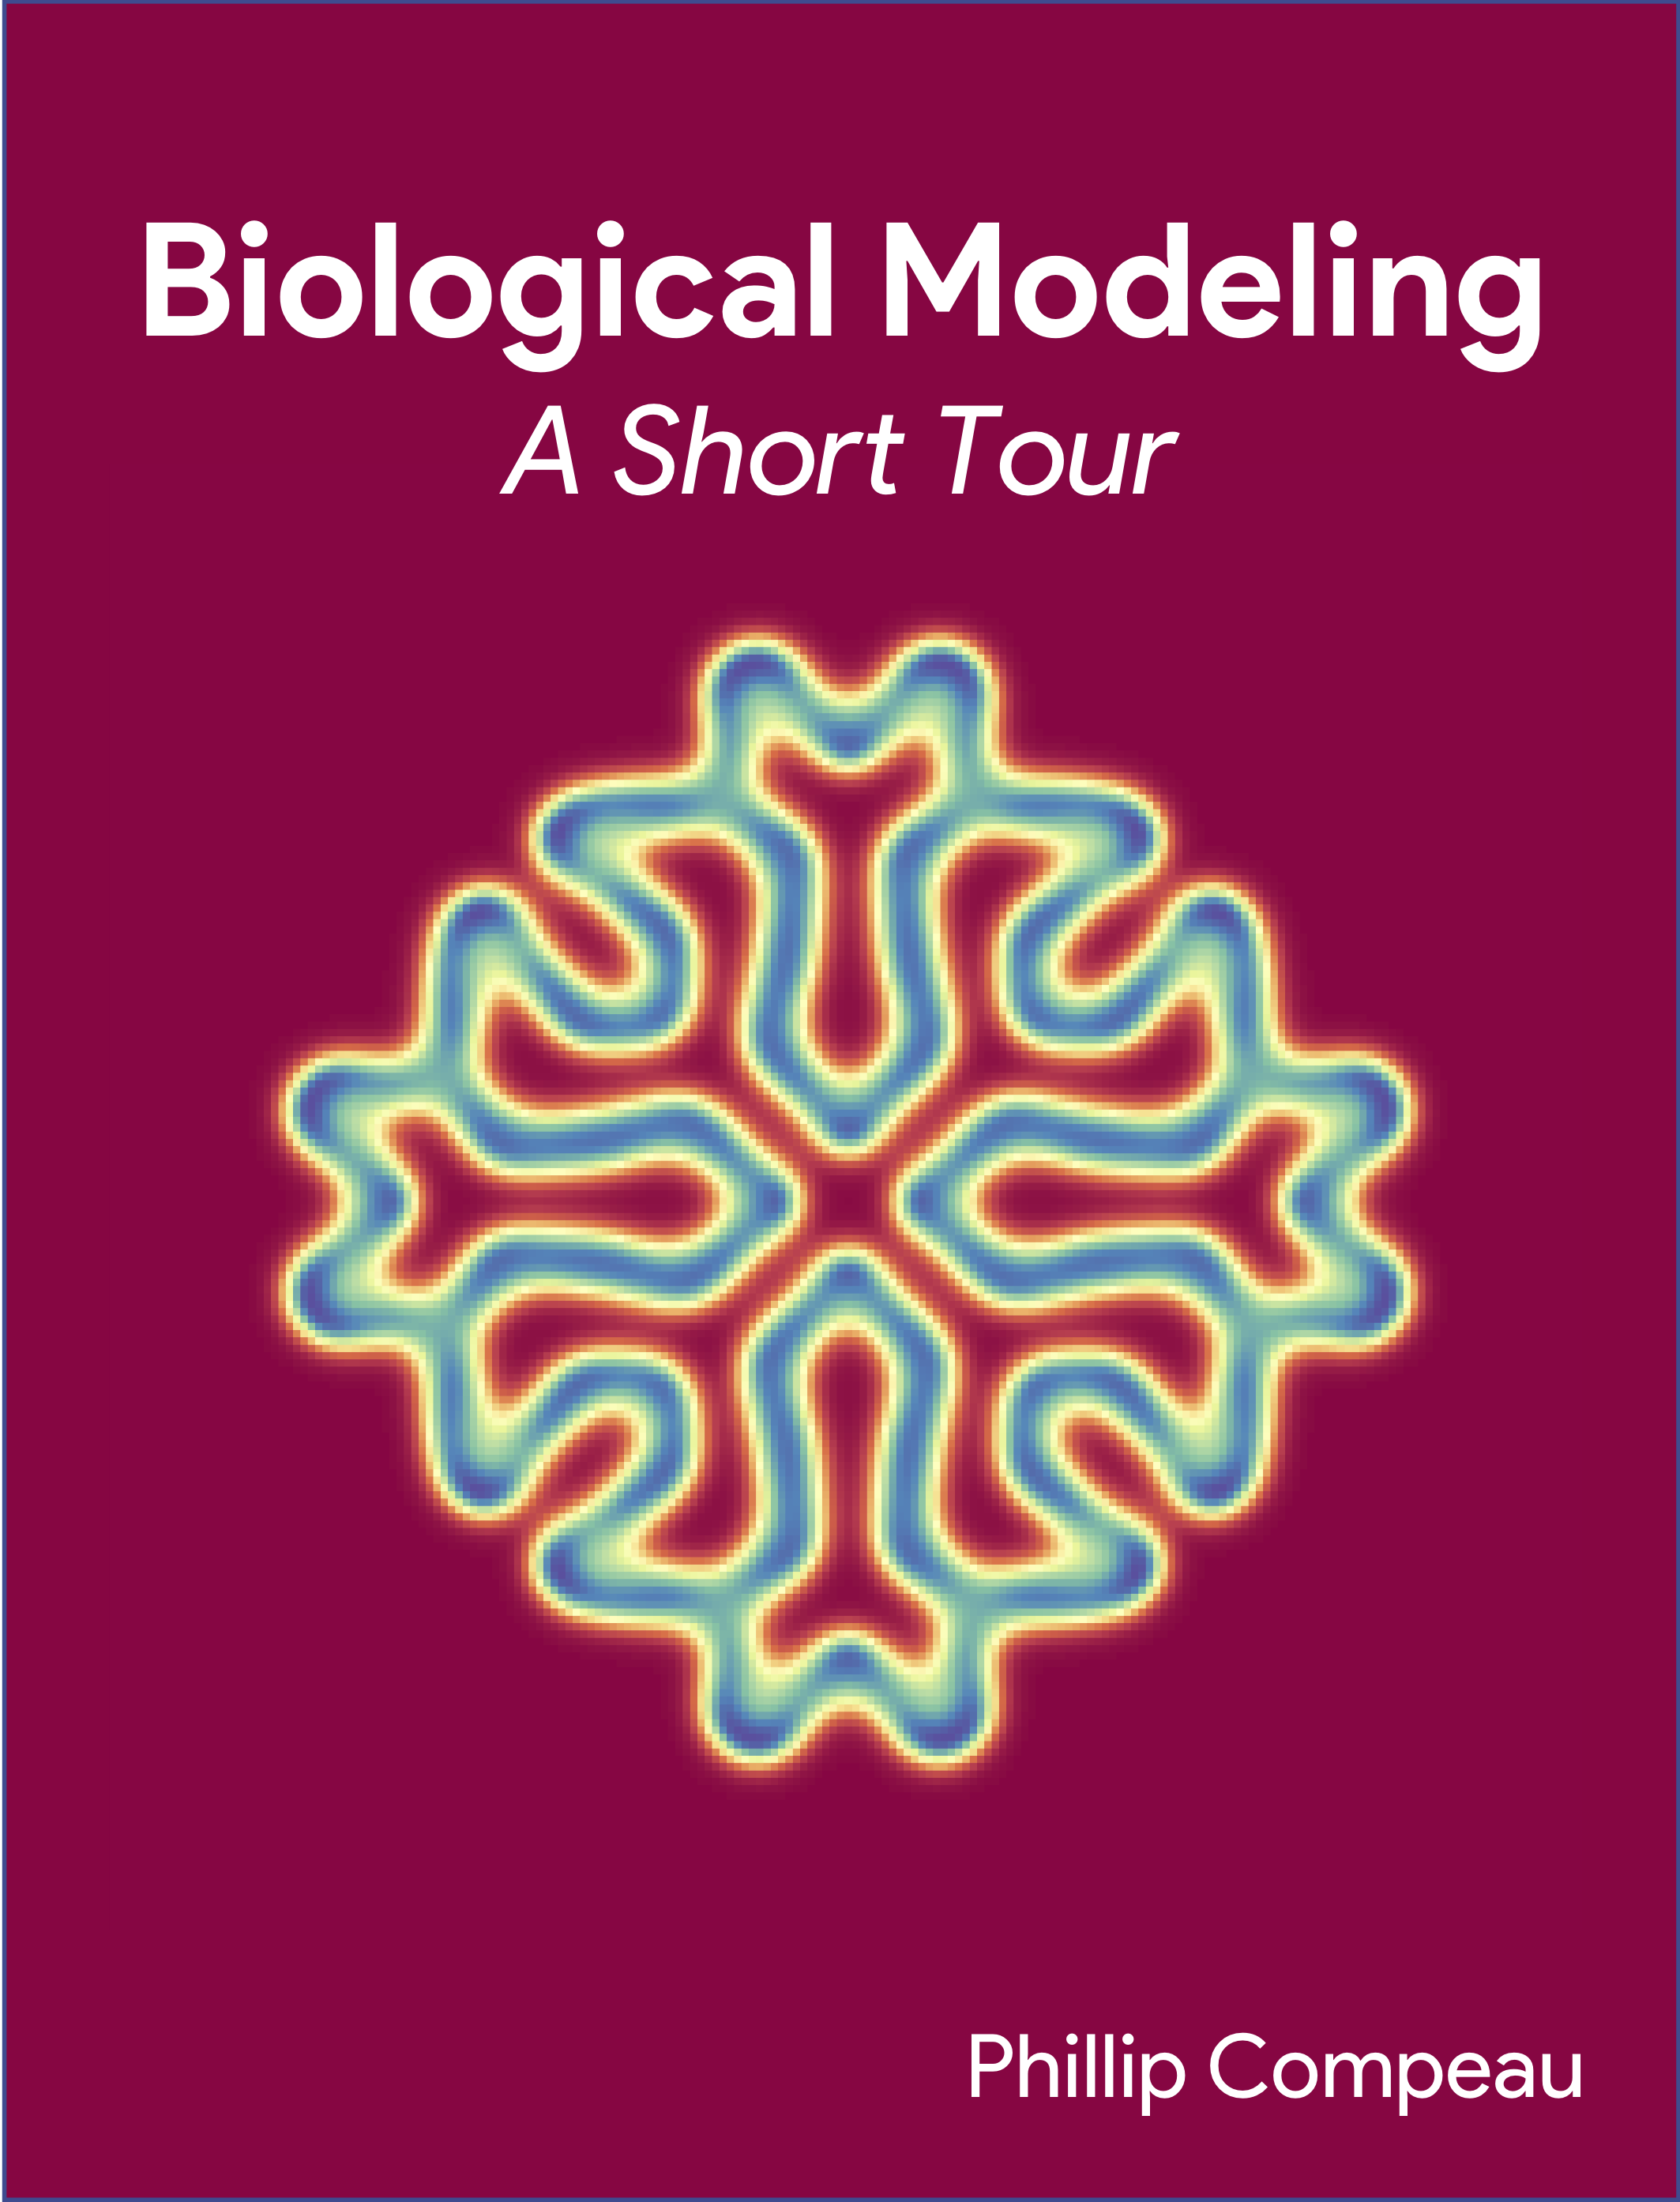
\includegraphics[width=\stockwidth]{../images/front_cover}}
}
\addtocounter{page}{-1}

\clearpage

% Title page

\clearpage\null
\thispagestyle{empty}
\AddToShipoutPictureBG*{% Add picture to current page
  \AtStockLowerLeft{% Add picture to lower-left corner of paper stock
    \includegraphics[width=\stockwidth]{../images/cover_page}}
}
\addtocounter{page}{-1}

\newpage


\thispagestyle{empty}

% Reverse title page

\phantom{}\vspace{17\baselineskip}

\noindent Copyright ©~2022 by Phillip Compeau. All rights reserved.\\

\noindent This book or any portion thereof may not be reproduced or used in any manner whatsoever without the express written permission of the publisher except for the use of brief quotations in a book review.\\

\noindent Printed in the United States of America\\

\noindent First Printing, 2022\\

\noindent ISBN: TBA\\

\noindent Library of Congress Control Number: TBA\\

\noindent Philomath Press, LLC\\
Pittsburgh, PA
\addtocounter{page}{-1}


\begin{dedication}
\textit{For Sandy Nichols, who taught me that mathematics might give me answers, but that writing would always keep me asking questions.}\\[\baselineskip]
\thispagestyle{empty}
\end{dedication}

\newpage
\phantomsection

% Blank page
\addtocounter{page}{-1}

% Welcome

\newpage
\phantomsection
\chapter{Welcome!}

Have you ever wondered why zebras have stripes? How your cells can quickly react to their environment and perform complex tasks without intelligence? Why the original SARS coronavirus fizzled out but SARS-CoV-2 has spread like wildfire around the planet? How algorithms can be trained to ``see'' cells as well as a human?

What all these questions share is that they can be answered by modeling biological systems at multiple ``scales'' of resolution, from the microscopic to the molecular. We will build models of biological systems that are relatively simple but nevertheless provide us with deep, fascinating insights into how those systems operate. Whether you are a biologist seeking to learn more about modeling, a mathematician or computer scientist hoping to see how quantitative methods can help us understand how biological systems work, or just a lover of science, we think you are in the right place.

This book is the print companion to \href{https://biologicalmodeling.org}{\textit{Biological Modeling}} (\href{https://biologicalmodeling.org}{biologicalmodeling.org}), a free and open online course teaching how to model biological systems at multiple scales. At the course website, you will find the full text of this book alongside a collection of tutorials walking you through how to build the models that we have used to reach our conclusions. Every time we encounter a tutorial, you will see the laptop symbol in the margin; if you are reading this as an ebook, then clicking on the laptop will take you directly to the relevant tutorial.\tutorial[]

These tutorials are built using the flagship software of the National Center for Multiscale Modeling of Biological Systems (MMBioS), a multi-university project. Although we use additional software where needed, each chapter is paired with a primary MMBioS software resource: \autoref{chapter:turing} and \autoref{chapter:motifs} are powered by MCell and CellBlender (\url{mcell.org}); \autoref{chapter:chemotaxis} is powered by BioNetGen (\url{bionetgen.org}); \autoref{chapter:coronavirus} is powered by ProDy (\url{http://prody.csb.pitt.edu}) and affiliated software; and \autoref{chapter:white_blood_cells} is powered by CellOrganizer (\url{cellorganizer.org}).

Each chapter has a collection of exercises at its end, many of which ask you to apply what you have learned to build your own models, but we also have integrated a collection of shorter ``STOP'' questions into the main text that invite you to check your understanding or contemplate the current material before continuing to the next topic. We also have ``Notes'' that provide short asides from the main text for readers who are interested.

Finally, this project may be the labor of love of a single person, but it is far from a solo effort. Every chapter in this book was co-authored by an undergraduate or master's student at Carnegie Mello Universityn. After the table of contents, we have short introductions of the talented team members who helped bring this book to life.

Thank you for joining us. We hope that you enjoy our little tour of biological modeling.

\begin{flushright}
\textit{Phillip Compeau}\\
\textit{Pittsburgh, PA}
\end{flushright}

\phantom{}\vspace{7.7\baselineskip}

\newpage

\nop{contents}{}
\tableofcontents*
\clearpage
\phantomsection


\newpage
\phantomsection
\chapter{Meet the Team}

\noindent\begin{tabular}{l @{\hskip 3em} l}
\parbox{0.28\textwidth}{\noindent \href{http://compeau.cbd.cmu.edu}{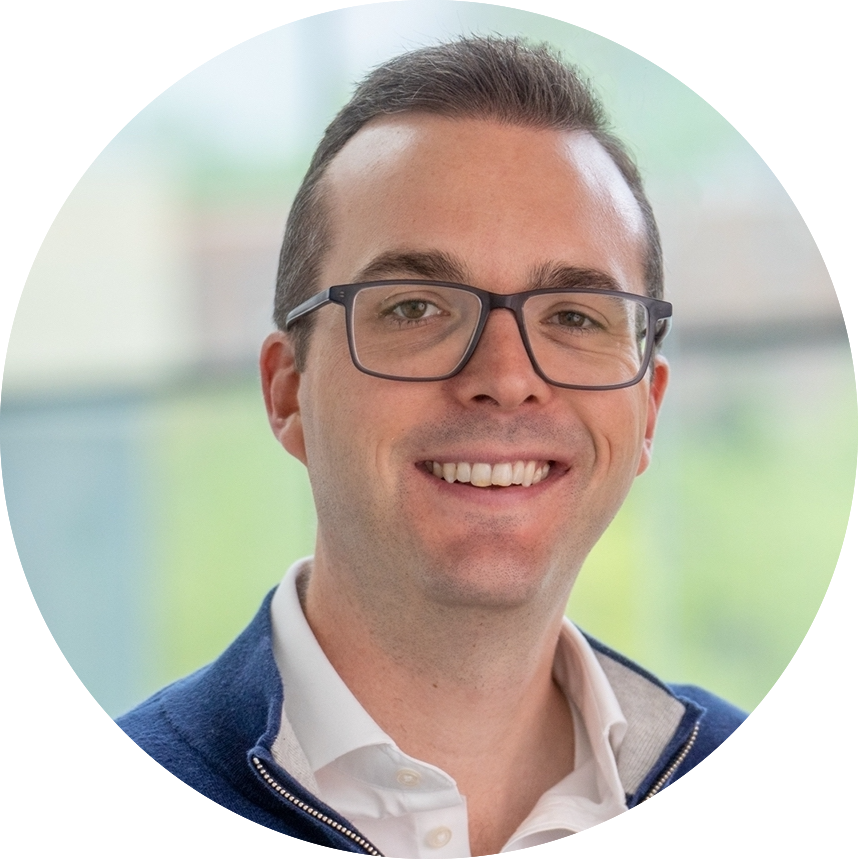
\includegraphics[width=0.28\textwidth]{../images/compeau_phillip_circle}}} & \parbox{0.7\textwidth}{\noindent {\small \href{http://compeau.cbd.cmu.edu}{\textbf{\textsc{Phillip Compeau}}} is the founder of \textit{Biological Modeling}. He is an Associate (Teaching) Professor and the Assistant Department Head in the Computational Biology Department at Carnegie Mellon University, where he directs the undergraduate program and co-directs the precollege program in computational biology. His online education projects, including \href{http://rosalind.info}{Rosalind}, \href{https://programmingforlovers.com}{Programming for Lovers}, and the \href{https://www.coursera.org/specializations/bioinformatics}{Bioinformatics Specialization} on Coursera, have reached over a million people. He is also the co-author of \textit{Bioinformatics Algorithms: An Active Learning Approach}, which has been adopted by 200 instructors in 45 countries.}}\\[22ex]

\parbox{0.28\textwidth}{\noindent \href{http://merterm.github.io}{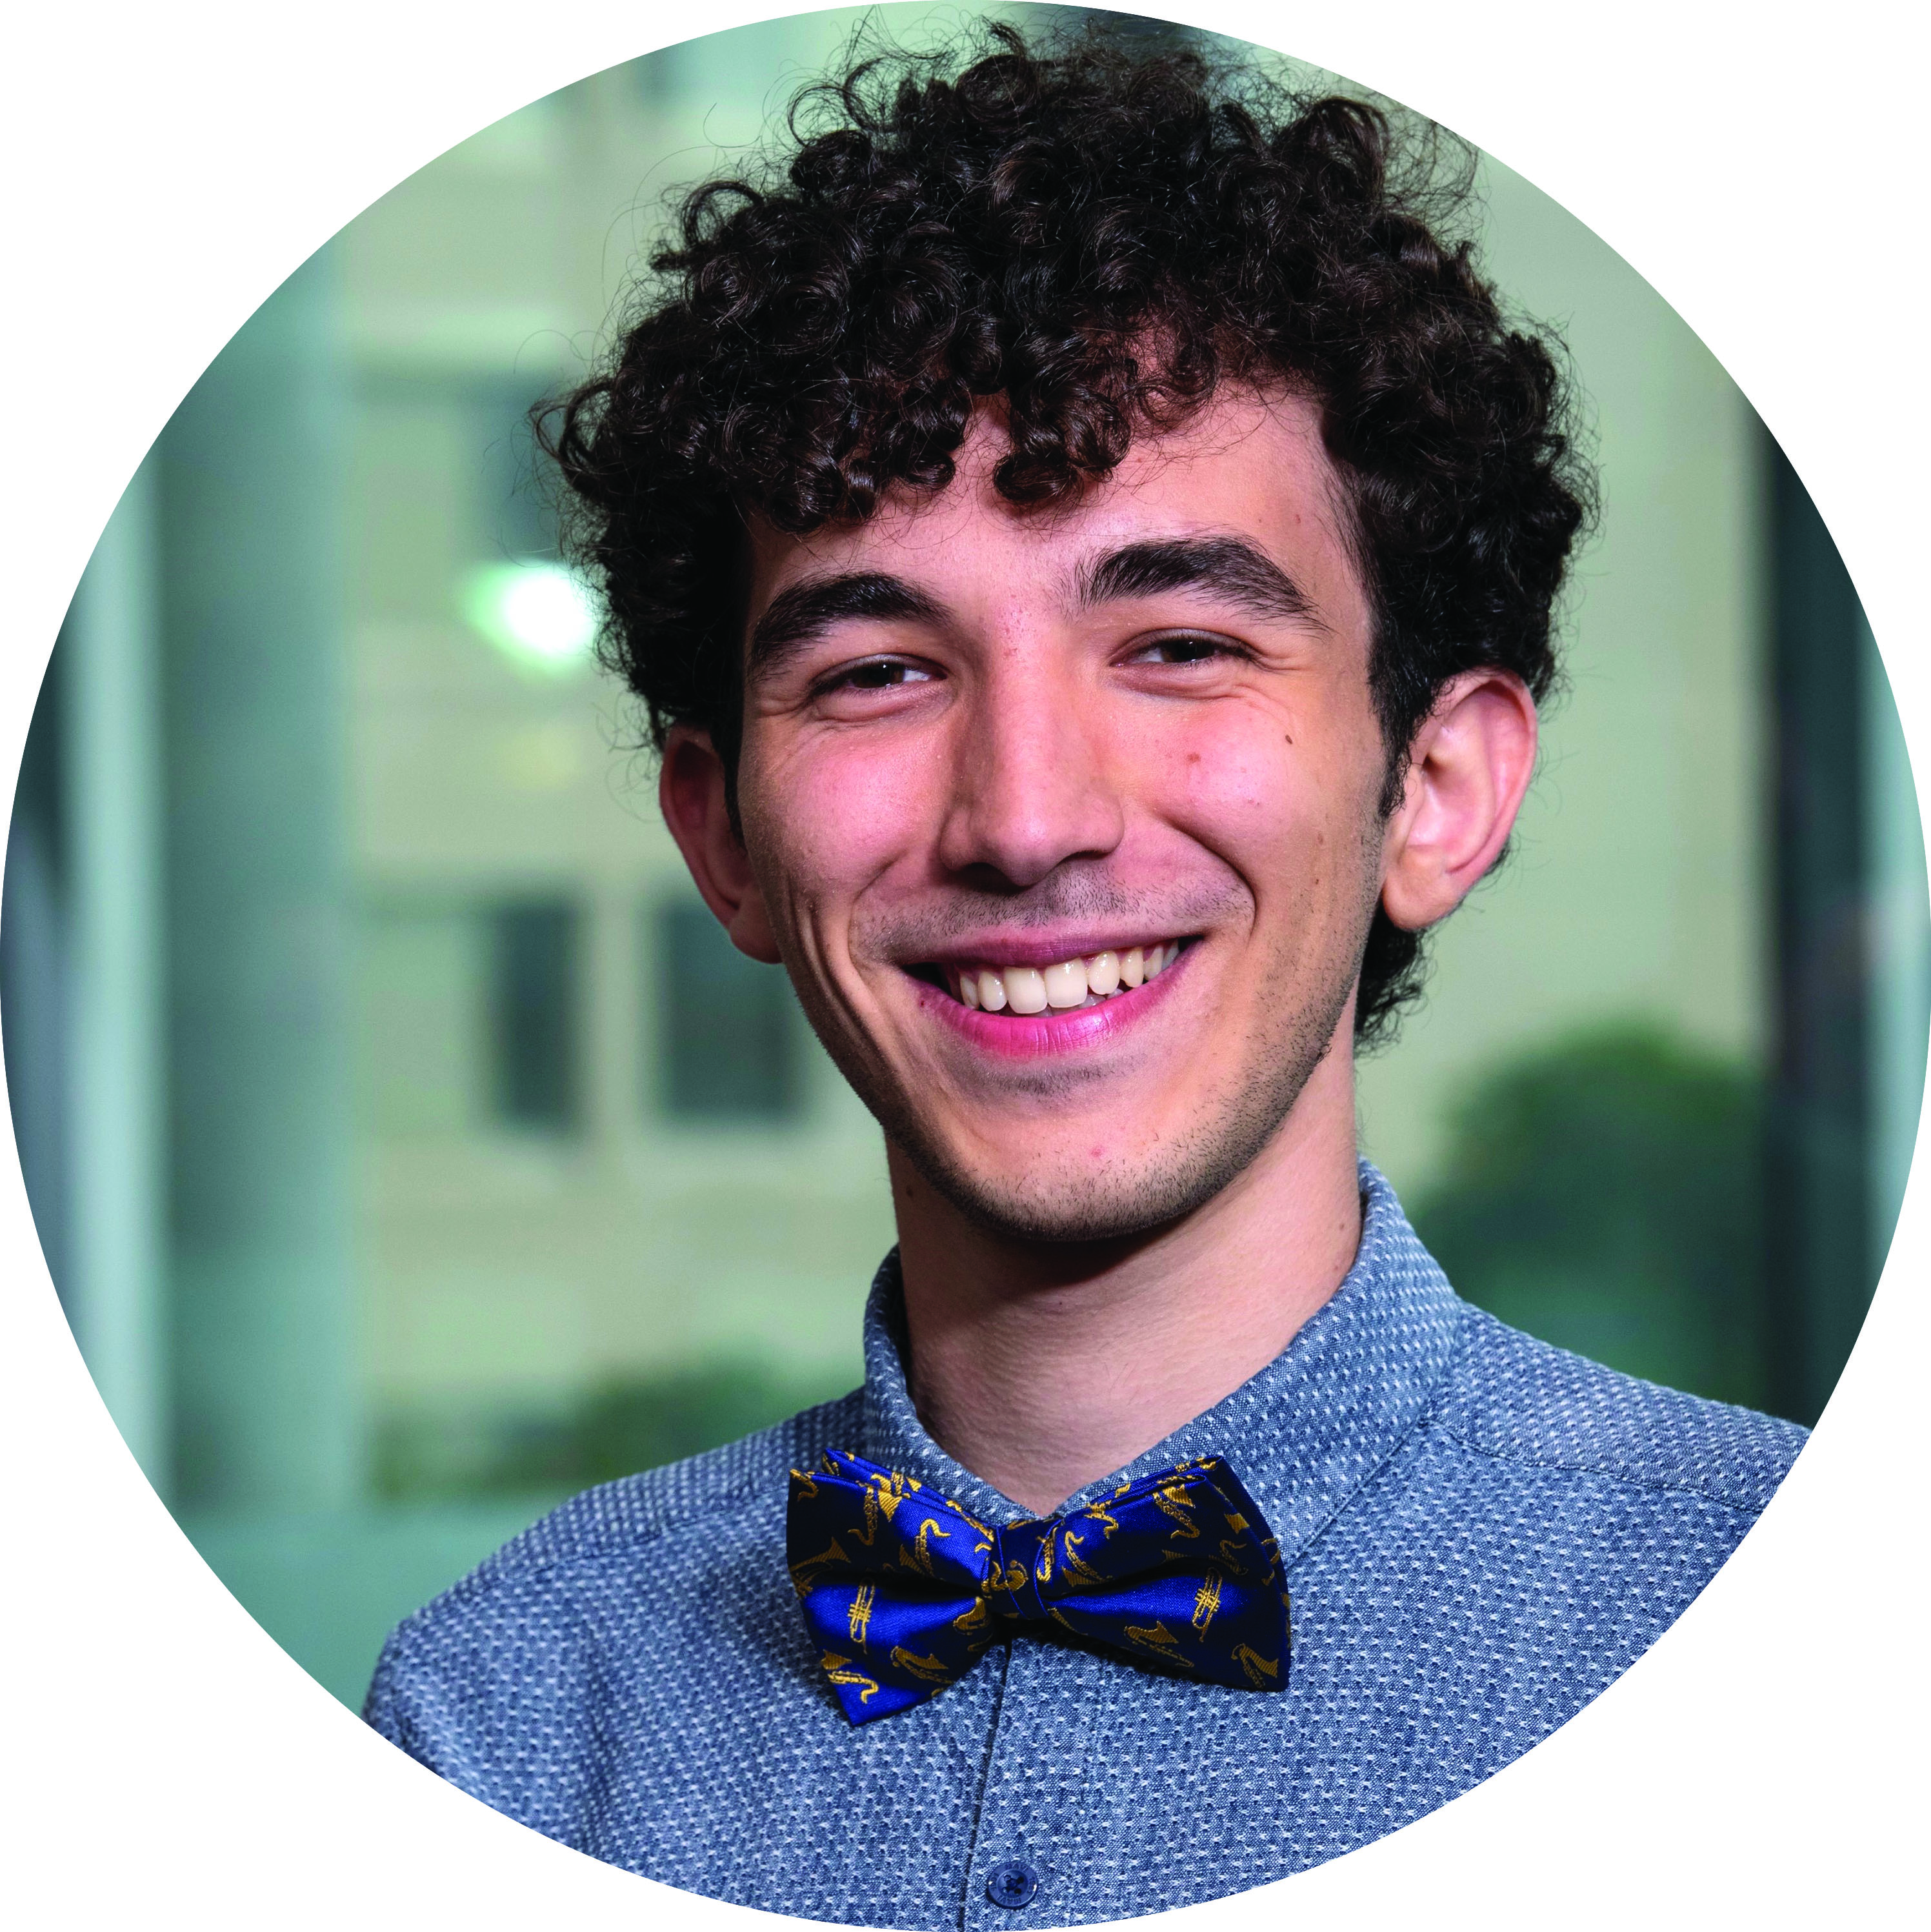
\includegraphics[width=0.28\textwidth]{../images/inan_mert_circle}}} & \parbox{0.7\textwidth}{\noindent {\small \textbf{\textsc{Mert Inan}} is a computer science Ph.D. student at the University of Pittsburgh and an alum of the M.S. in computational biology program at Carnegie Mellon University. He loves interdisciplinary fields and has been working at the intersection of computation, biology, neuroscience, and machine intelligence. Unlocking the secrets of biology is a pleasure that Mert truly enjoys.}}
\end{tabular}

\noindent\begin{tabular}[m]{l @{\hskip 3em} l}
\parbox{0.28\textwidth}{\noindent \href{https://cbb.yale.edu/people/noah-yann-lee}{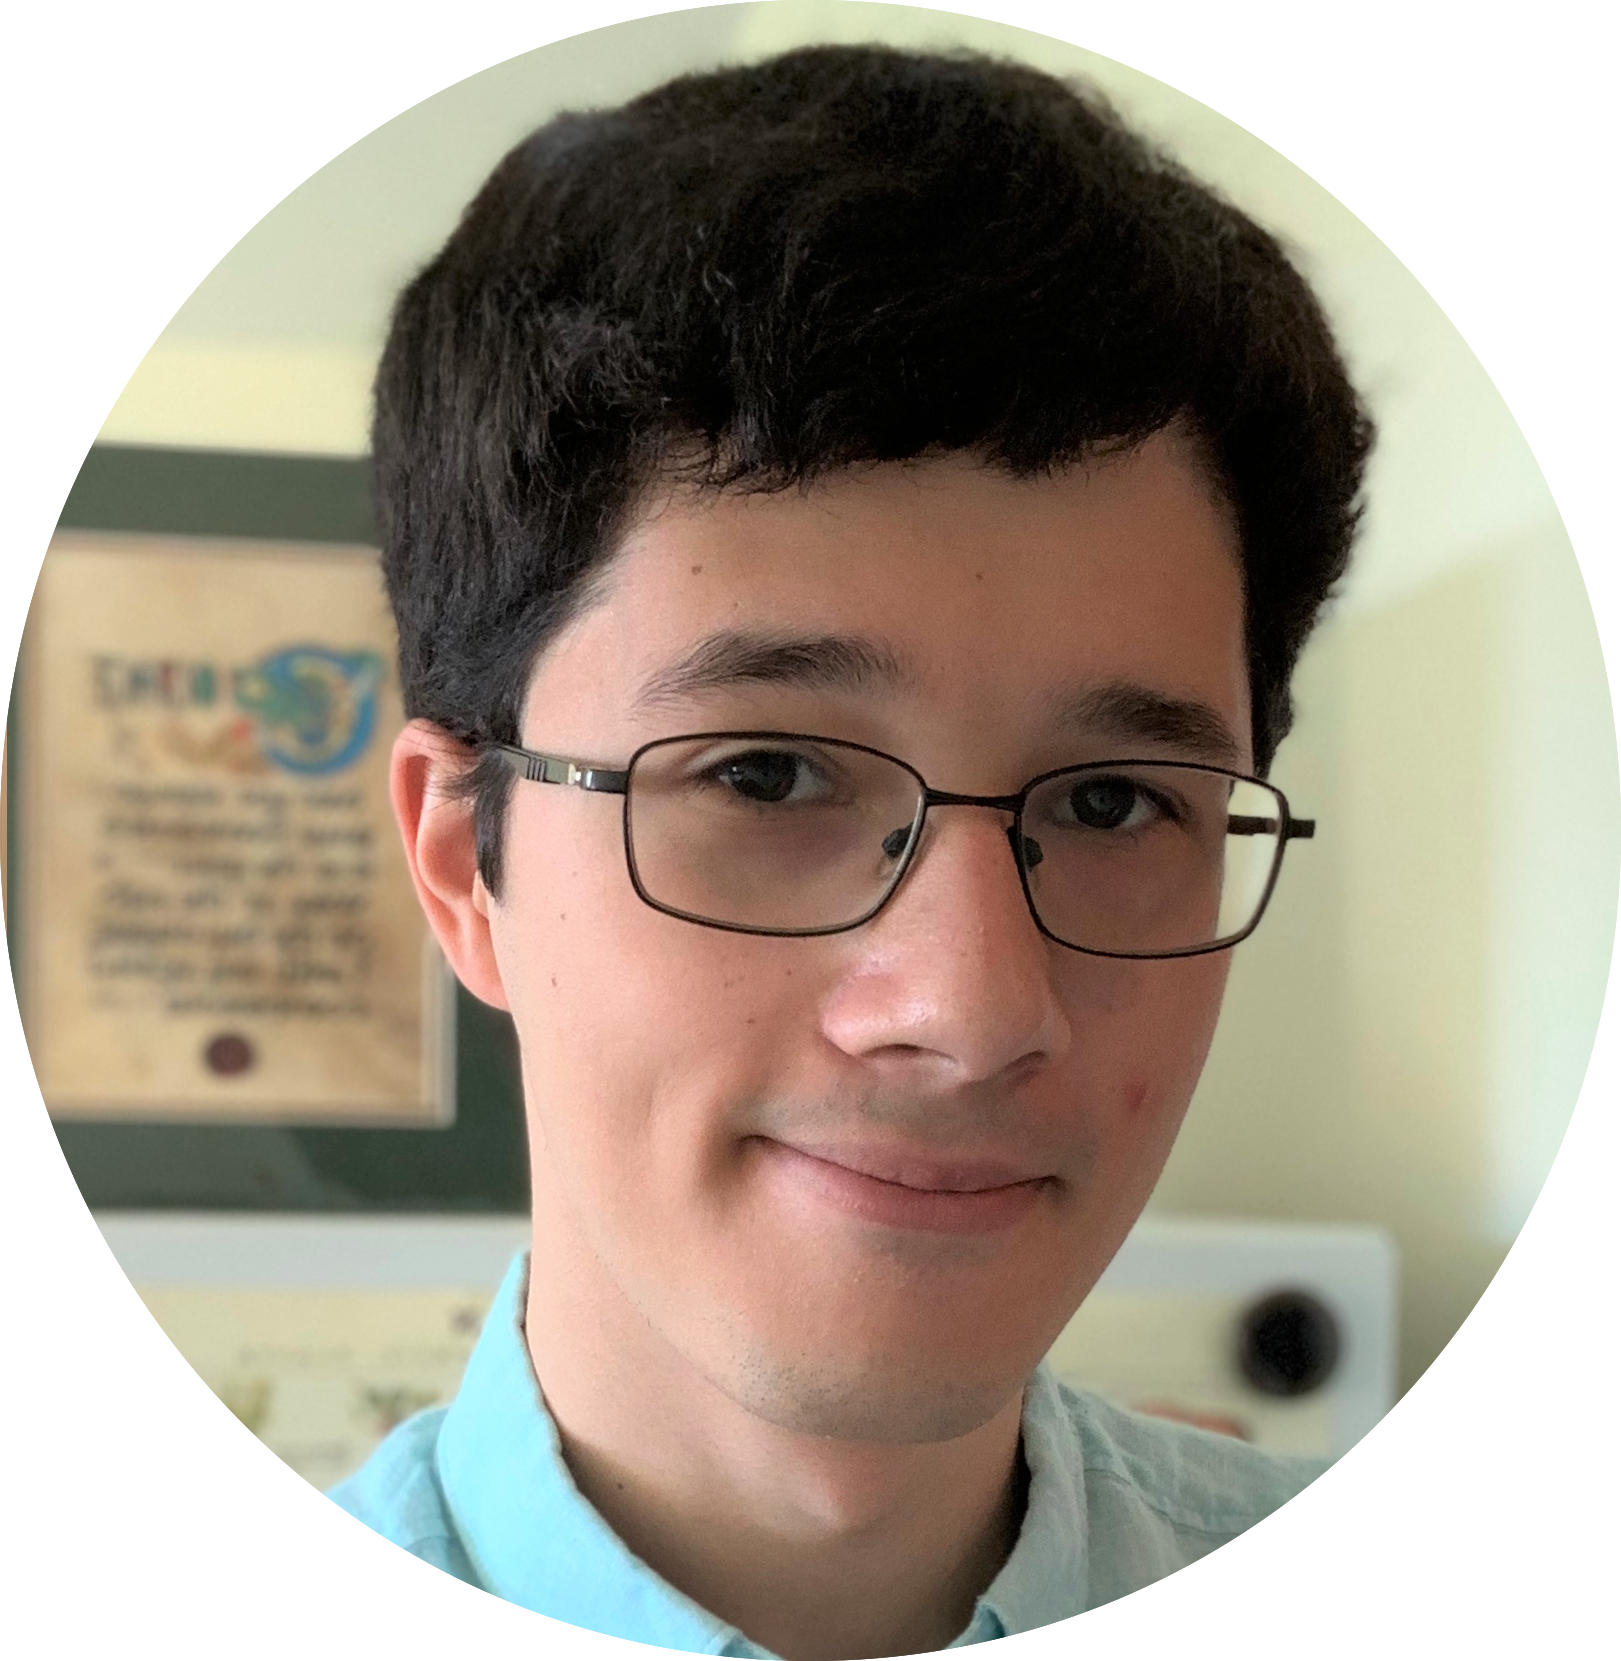
\includegraphics[width=0.28\textwidth]{../images/lee_noah_circle}}} & \parbox{0.7\textwidth}{\noindent {\small \textbf{\textsc{Noah Yann Lee}} is a PhD student at Yale University in the Computational Biology and Bioinfornatics program and an alum of the undergraduate program in computational biology at Carnegie Mellon University. From running early-childhood educational tests with the Children’s School at Carnegie Mellon for the Global Learning XPRIZE, to cultivating and sequencing phage genomes with the PhageHunters program, Noah has an appreciation for science from the micro to the macro, physical to the digital. Noah is interested in projects and organizations working with STEM education, and science outreach.}}\\[22ex]

\parbox{0.28\textwidth}{\noindent \href{https://www.linkedin.com/in/chris-lee-b1a020158/}{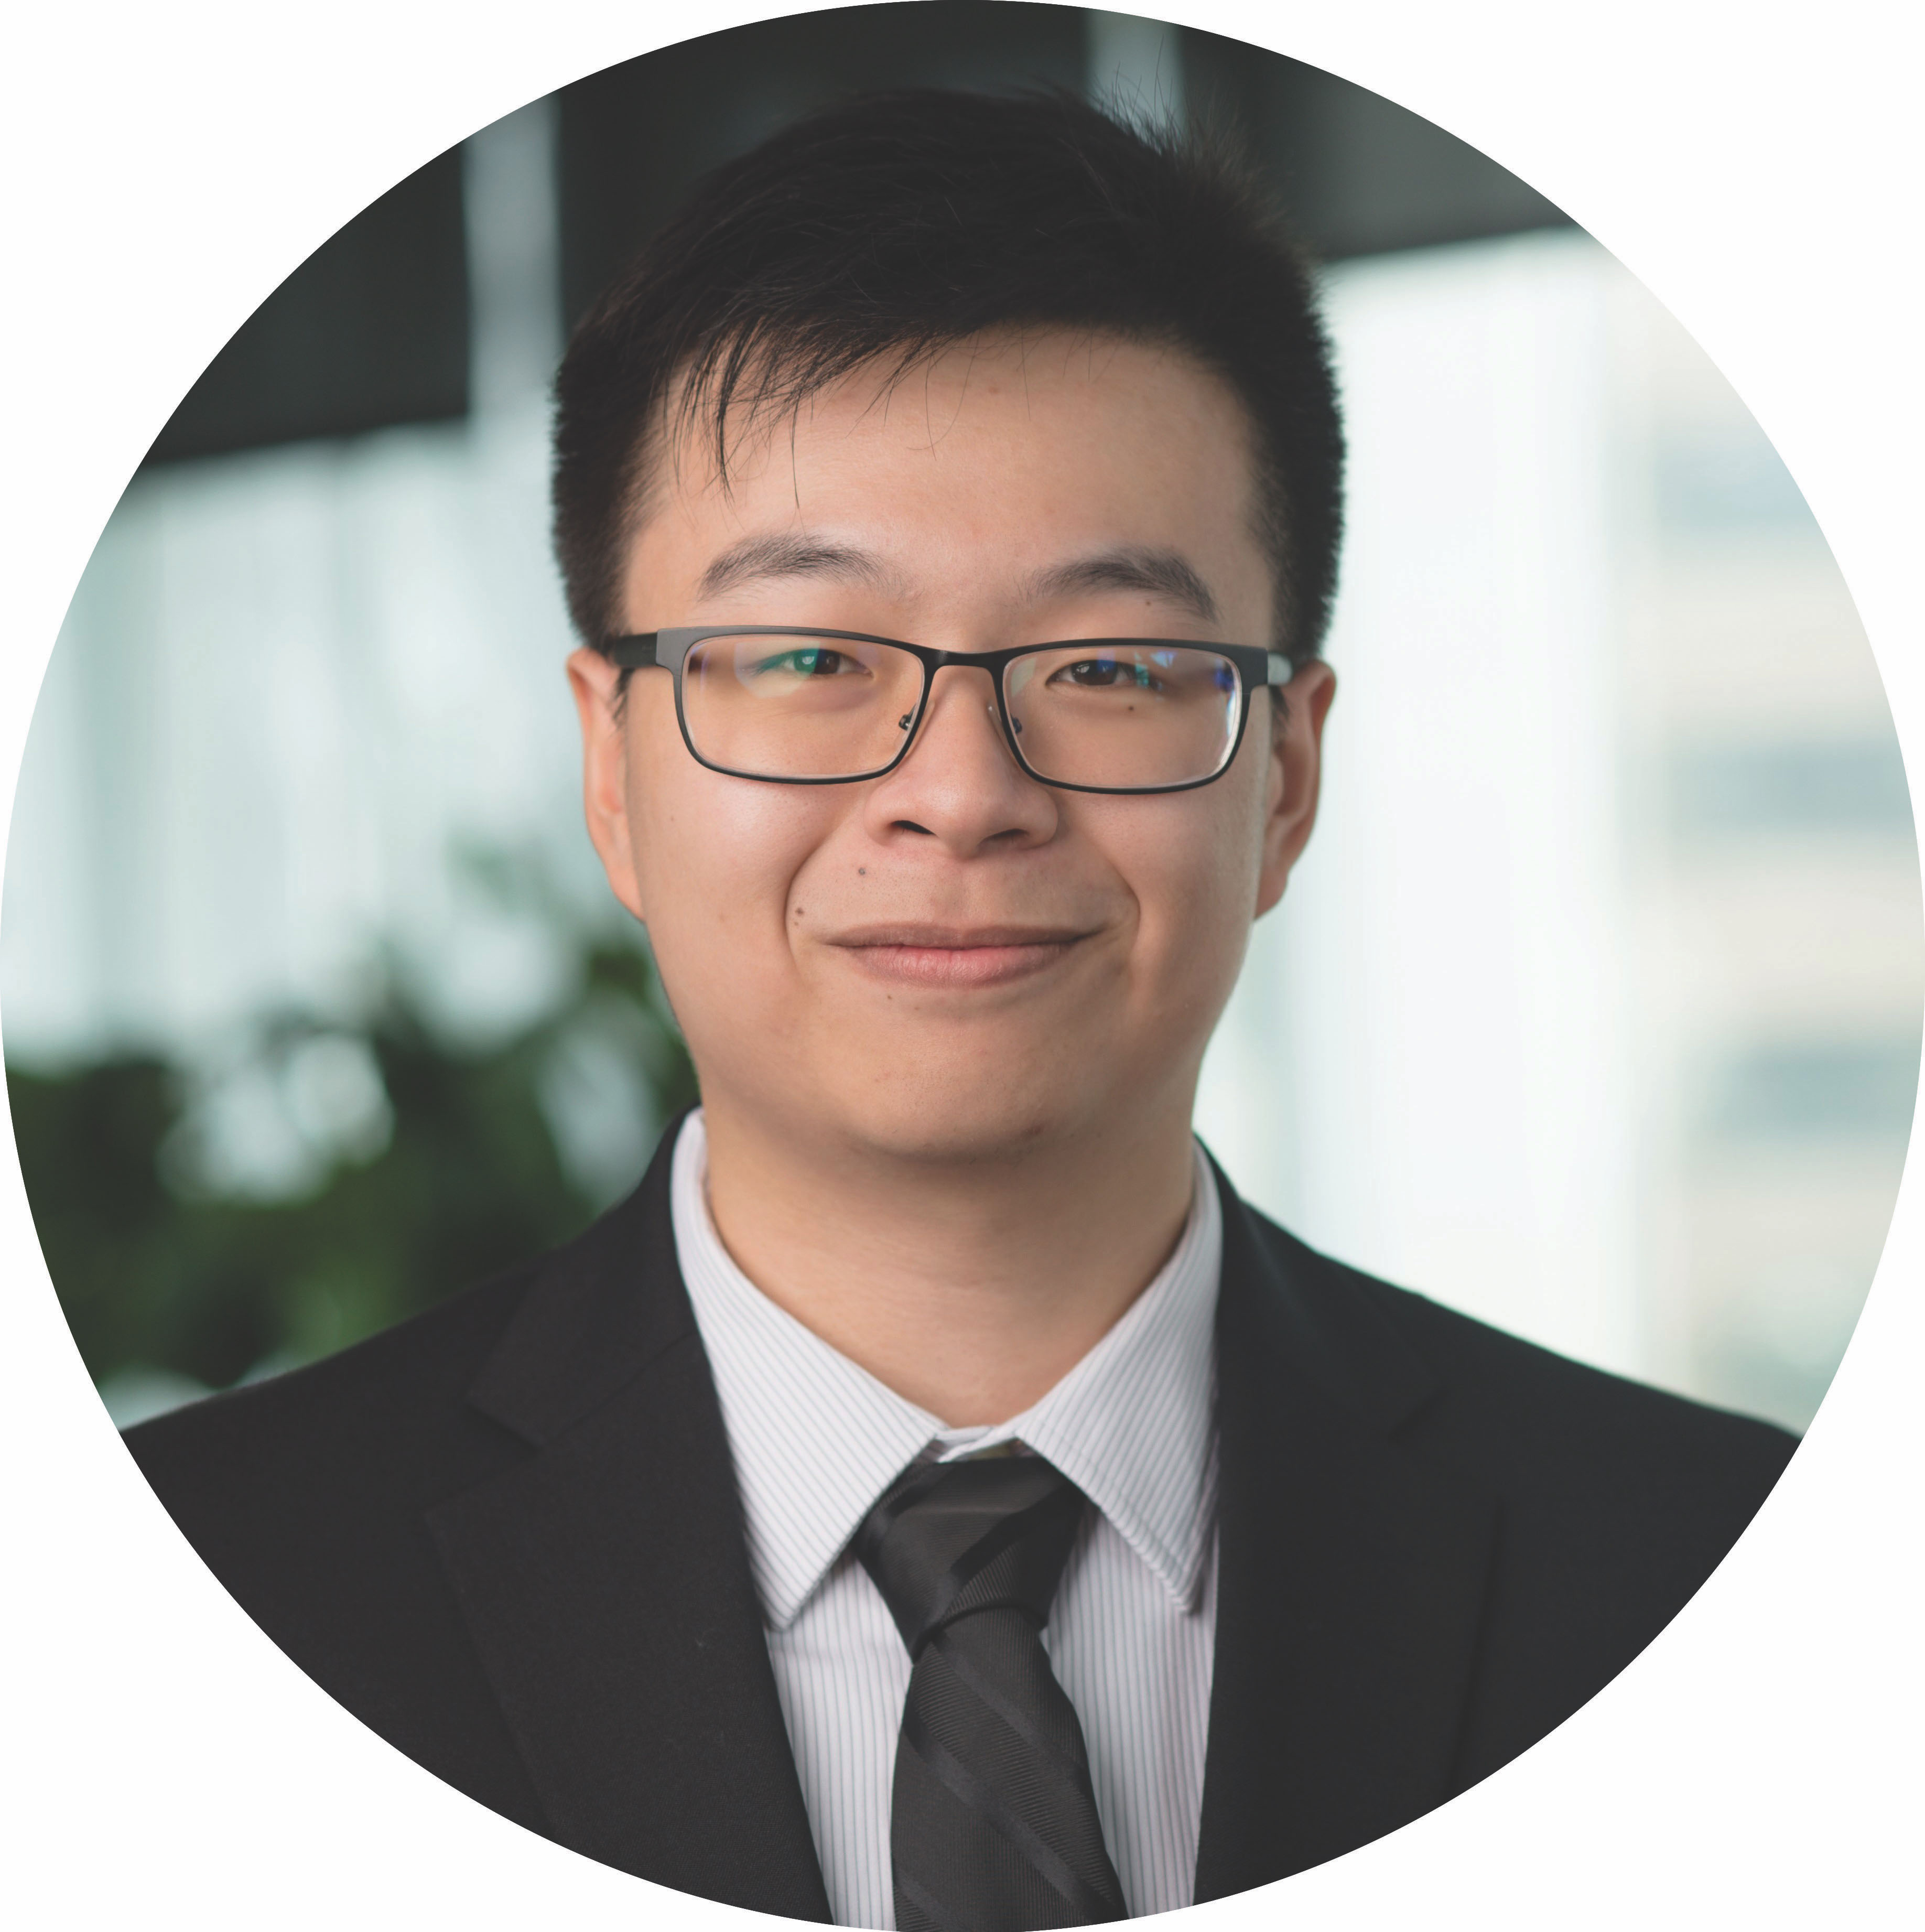
\includegraphics[width=0.28\textwidth]{../images/lee_chris_circle}}} & \parbox{0.7\textwidth}{\noindent {\small \textbf{\textsc{Chris Lee}} is an associate computational biologist at Dicerna Pharmaceuticals. He is an alum of the M.S. in Computational Biology at Carnegie Mellon University; previously, he was an undergraduate student at Rutgers University and worked as an undergraduate researcher studying hydrothermal vent bacteria, where he graduated magna cum laude with a B.A. in Molecular Biology \& Biochemistry and double minor in Chemistry and Computer Science.}}\\[20ex]

\parbox{0.28\textwidth}{\noindent \href{https://www.linkedin.com/in/shuanger-li-38b300133/}{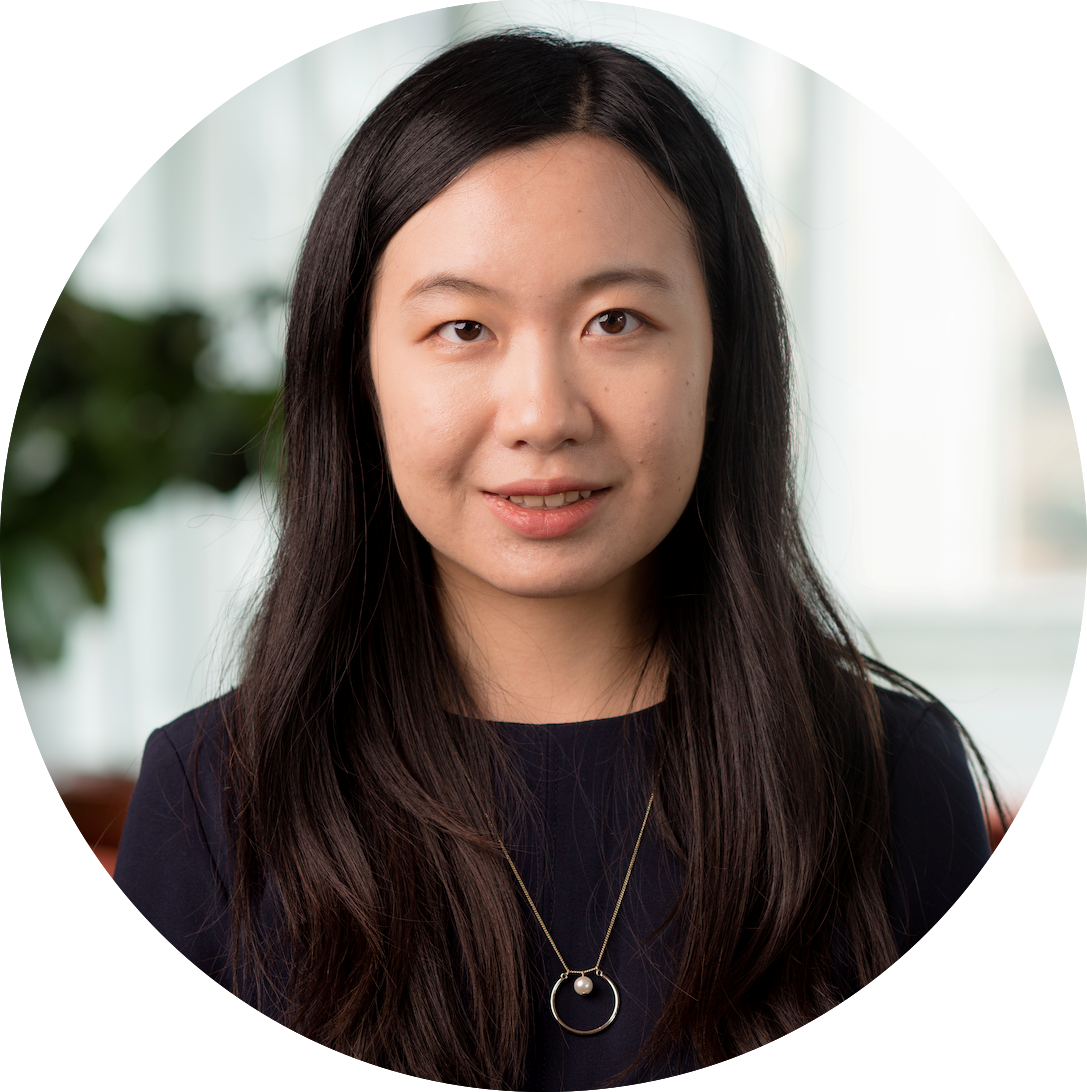
\includegraphics[width=0.28\textwidth]{../images/li_shuanger_circle}}} & \parbox{0.7\textwidth}{\noindent {\small \textbf{\textsc{Shuanger Li}} is a PhD student at the University of Chicago, and an alum of the M.S. in Computational Biology at Carnegie Mellon, where she worked with Dr. Oana Carja on heritable phenotypic variability. She enjoys modeling and simulation as powerful and fun ways to understand biological systems. She double majored in Environmental Sciences and Microbial Biology at UC Berkeley, where she studied Hawaiian arthropod assemblages, spider behaviors, and remediation bioreactors.}}\\

\end{tabular}

\newpage

%\twitter[http://www.twitter.com/phillipcompeau]
%\linkedin[http://www.linkedin.com/in/phillipcompeau/]{0}

 
\clearpage
\phantomsection
\chapter{Acknowledgments}
\label{chapter:acknowledgments}

The online course from which this book derives, \href{https://biologicalmodeling.org}{\textit{Biological Modeling}}, is a training and dissemination effort for the National Center for Multiscale Modeling of Biological Systems (MMBioS). The development of that course has been supported by the National Institutes of Health (grant ID: P41 GM103712).

We would like to thank everyone who has contributed to the development of MMBioS software, as their work allowed this project to come about. We also would like to thank the other members of our training and dissemination team (Alex Ropelewski, Joe Ayoob, and Rozita Laghaei) as well as the Director of MMBioS, Jim Faeder.

We are grateful to Nicole Matamala, who helped develop tutorials for \autoref{chatper:white_blood_cells}, Yanjing Li, who helped develop exercises for \autoref{chapter:white_blood_cells}, and Velasquez Ebanks and Ulani Qi, who helped work on an early version of \textit{Biological Modeling}. Special thanks to Adam Mihalik, who provided helpful comments on an early draft of this work.

\autoref{chapter:motifs} was in part inspired by Uri Alon’s research and superlative textbook \href{https://www.weizmann.ac.il/mcb/UriAlon/introduction-systems-biology-design-principles-biological-circuits}{\textit{An Introduction to Systems Biology}}, a classic that we strongly recommend if you are interested in a greater discussion of biological network motifs.

Finally, and most importantly, the publication of this book was graciously crowdfunded on \href{https://www.kickstarter.com/projects/phillipcompeau/biological-modeling-a-short-tour?ref=user_menu}{Kickstarter}. As part of the campaign, a number of individuals showed their support above and beyond anything we could have ever imagined. As a token of our eternal gratitude, we are listing them below.
\begin{center}
\tabcolsep=2em
\begin{tabular}{l l}
Rumi Naik & Jill Gunn\\
Nicole Fontanese & Thomas Hutchinson Castro\\
Johnathon Nicolas Roman & Coralline Oz\\
Gillian Hawketts & Robert Lucyshyn\\
Ben Mescher & Jack and Will Haselhorst\\
Dave Lemen & Kevin Mai\\
Emily Tu & Othman Soufan\\
Suraj Nair & Joel Rodriguez Medina\\
Michael Li & Jason Dass\\
Austin Boucinha, OCT & Martin\\
Mark Mammel & Akash Ramachandran\\
Will Townes & Darrell Thomas\\
Sean Leonard & Eric Song\\
Hal Snyder & Jared A.~Davis\\
Kevin Reed & Roger Walker\\
Maxwell Shapiro & Jérémie Sartor\\
Jeff Buck & Christopher James Langmead\\
Jacqueline McVeigh & Nikolett Lehel Lassie\\
Kelly Johnson & Jonathan McMenamin-Balano\\
Sassy Momassy & Mary B.~Kennedy\\
William S Owen & HD Welker\\
Wayne Myers & Adam Mihalik\\
Luther Tweneboah Evans & Braden Kartchner\\
Christos Noutsos & Costel Radu\\
Michael Levy & Leeza Sergeeva\\
Genene Hayes & Steven Fines\\
Jonathan M. & Gary L.~Keyfauver, PhD\\
Avinash Seetharamaiah & Steve Ross\\
Laura Climer & Joshua Coleman\\
Jim Reesman & Defne Surujon\\
Nick Connors & Pavel Pevzner\\
\end{tabular}
\end{center}

%
%\noindent This textbook was greatly improved by the efforts of a large number of individuals, to whom we owe a debt of gratitude.
%
%The development team, as well as Laurence Bernstein, Ksenia Krasheninnikova, Max Shen, and Jeffrey Yuan, implemented coding challenges and exercises, rendered figures, helped typeset the text, and offered insightful feedback on the manuscript.
%
%Glenn Tesler provided thorough chapter reviews and even implemented some software to catch errors in the early version of the manuscript!
%
%Robin Betz, Petar Ivanov, James Jensen, and Yu Lin provided insightful comments on the manuscript in its early stages. David Robinson was kind enough to copy edit a few chapters and palliate our punctuation maladies.
%
%Randall Christopher brought to life our crazy ideas for illustrations throughout the book, including the chapter header cartoons and the textbook cover.
%
%Andrey Grigoriev and Max Alekseyev gave advice on the content of \autoref{chapter:replication} and \autoref{chapter:rearrangements}, respectively. Martin Tompa helped us develop the narrative in \autoref{chapter:motifs} by suggesting that we analyze latent tuberculosis infection.
%
%Nikolay Vyahhi led a team composed of Andrey Balandin, Artem Suschev, Aleksey Kladov, and Kirill Shikhanov, who worked hard to support an online, interactive version of this textbook used in our online courses on Coursera.
%
%Our students on Coursera, especially Mark Mammel, Isabel Lupiani, Erika Ram\'irez and Dmitry Kuzminov, found hundreds of typos in our preliminary manuscript.
%
%Mikhail Gelfand, Uri Keich, Hosein Mohimani, Son Pham, and Glenn Tesler advised us on some of the book's ``Open Problems'' and led Massive Open Online Research projects (MOORs) in the first session of our online course.
%
%The Big Data to Knowledge Program at the National Institutes of Health, as well as Howard Hughes Medical Institute and the Russian Ministry of Education and Science generously gave their support for the development of the online courses accompanying this textbook.  The Bioinformatics and Systems Biology Program and the Computer Science \& Engineering Department at the University of California, San Diego provided additional support.
%
%Finally, our families gracefully endured the many long days and nights that we spent poring over manuscripts over the last several years; they helped us preserve our sanity along the way.
%
%\vspace{\baselineskip}
%
%\begin{minipage}{\textwidth}
%\raggedleft\noindent\parbox{0.18\textwidth}{\raggedright\itshape P.\,C. and P.\,P.\\
%May 2018
%}
%\end{minipage}

\newpage \phantom{}
\thispagestyle{empty}